\chapter{Improvements}
\label{chap:Improvements}
Multiple ideas were explored to improve the performance of PARSEC \cite{PARSEC_VD}.
This chapter describes each idea and its individual impact on overall performance.
All improvements are then combined to present the final results in Chapter \ref{chap:Results}.

The criteria used for quantifying the contributions of these improvements are the number of intersections performed and the total running time. These measures are reported as speedups. Formally, we define the intersection speedup and time speedup as:
$$
    \text{Intersection Speedup} = \frac{\text{\# of Intersections Baseline}}{\text{\# of Intersections New}}
$$
$$
    \text{Time Speedup} = \frac{\text{Run time Baseline}}{\text{Run time New}}
$$
The information of data graphs and queries used to report individual performance impact is mentioned in Section \ref{sec:expt-info}.

\section{Intersection Reuse}\label{sec:reuse-impl}
Adjacency list intersection operation for generating next candidates (Algorithm \ref{algo:intersect}) is the most time-consuming operation in subgraph enumeration.
This is a well-established fact in the literature \cite{RPS-paper}, \cite{LIGHT}, \cite{VF3} and it was also verified for the baseline \cite{PARSEC_VD}.
Figure \ref{fig:time-dist} presents the distribution of time spent by each operation in different tasks.
The Intersect operation shown here is the time taken by Algorithm \ref{algo:intersect}.
\begin{figure}
    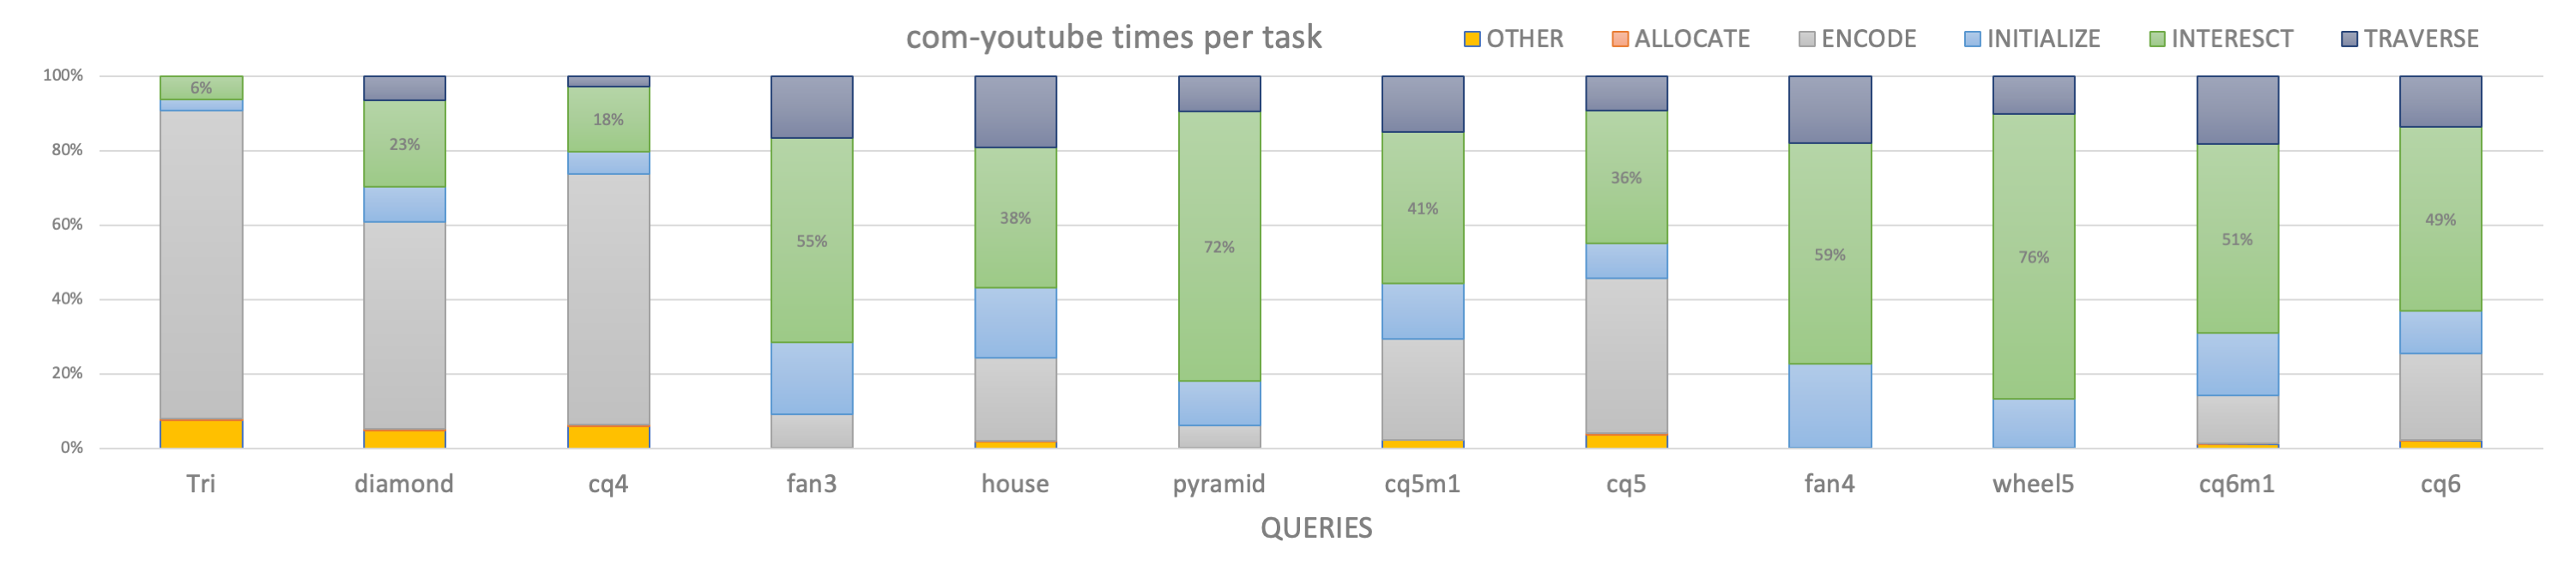
\includegraphics[width=\textwidth]{fig/improvements/time-distributions-yt.png}
    \caption{Stepwise fraction time spent}
    \label{fig:time-dist}
\end{figure}
This algorithm iterates over each element in the backward neighbors list to perform adjacency list intersection and generates possible candidates for next level (lines 2 - 5).
The size of the backward neighbors list increases for larger templates, which results in even more adjacency list intersections at each node.

RPS \cite{RPS-paper} reduces these operations by generating an intersection reuse plan which smartly finds the intersections that will be required by more than one node and stores them after first computation.
% There is a lot of intersection reuse possible with RPS as they employ a BFS strategy.
The authors report huge scope for intersection reuse through this plan.
However, most of the reuse opportunities arise due to BFS traversal.
A similar extent of reuse is not possible with DFS traversal since the information is lost while backtracking.
However, Some levels of the sequenced query graph have similar backward neighbor lists.
For such queries, some intersections can be reused by simply storing the intermediate intersection results.
To do this efficiently, one needs to match levels with similar adjacency lists.
This problem is posed as a linear programming optimization problem.

Let the sequenced query graph be $G_q=(V_q, E_q)$ with $|V_q|=k$ and the match order be $S_q$.
Let $\mathcal{N}(.)$ represent the backward neighbors list of a vertex.
For each vertex pair $S_q(i), S_q(j)$, let $W_{ij}$ be a measure of the commonality between their backward neighbors.
Let $X_{ij}$ be the variable which decides if vertex $i$ should reuse intersections from vertex $j$.

With these definitions the optimization problem can be modelled as:
\begin{align}
    \max \sum_{i=j+1}^{k}\sum_{j=1}^{k} W_{ij} X_{ij} \label{eq:obj} \qquad \qquad \\
    \text{s.t.}
    \sum_{j=1}^k X_{ij} \leq 1 \qquad \forall i \in \{1, \dots, k\} \label{eq:con1}
\end{align}
Where, $$
    W_{ij} = \begin{cases}
        |\mathcal{N}(S_q[i]) \cap \mathcal{N}(S_q[j])| \qquad \text{if } i>j,~\mathcal{N}(S_q[i]) \supseteq \mathcal{N}(S_q[j])  \text{, and} \\
        0   \qquad \text{otherwise.}
    \end{cases}
$$
The maximization problem (\ref{eq:obj} - \ref{eq:con1}) is a Linear Semi-Assignment Problem (LSAP) for which the greedy solution is optimal.
% This is easy to establish as any other solution can be improved by switching to the ÷greedy solution.
Hence, the solution is:
$$
    X_{ij}=\begin{cases}
        1   \qquad \text{if } j=\argmax_j(w_{ij}>0); \\
        0   \qquad \text{Otherwise}
    \end{cases}
$$
Reuse detection involves a maximum operation for each level in $G_q$ hence it is polynomial time and can be executed on the CPU for small-sized query graphs.
The mappings found ($x_{ij} = 1$) imply that level $i$ can use intersection results from level $j$.
Hence, level $j$ is flagged as \textit{reusable} and its intersection results are stored along with the DFS stack.
Algorithm \ref{algo:reuse} lists the reuse detection and post-processing recipe.
To save constant memory footprint, the query graphs are stored in CSR format.
After finding the reuse mappings, the column index of $(G_q)$ needs to be modified for efficient search tree traversal.
The modification step involves reordering the adjacency lists and generating the reuse pointer array.

We show reuse detection at work on the example query in Figure \ref{fig:sgm-example}.
Here, only $w_{54}$ and $w_{53}$ are positive with value 2. Hence, one from levels 3 or 4 can be marked reusable, let's assume level 4.
The backward neighbors of level 4 are $\{1,3\}$ and level 5 are $\{1,2,3\}$.
% A reuse pointer array is created to avoid checks inside the for loop of Algorithm \ref{algo:intersect} (line 2).
A reuse pointer array, that points to the start of the remaining neighbors of level 5 is created to avoid extra checks in Algorithm \ref{algo:intersect}.
% To avoid checks indie the for loop of Algorithm \ref{algo:intersect} (line 2), another Reuse pointer array is created which gives the start of the remaining neighbors of level 5.
\begin{figure}
    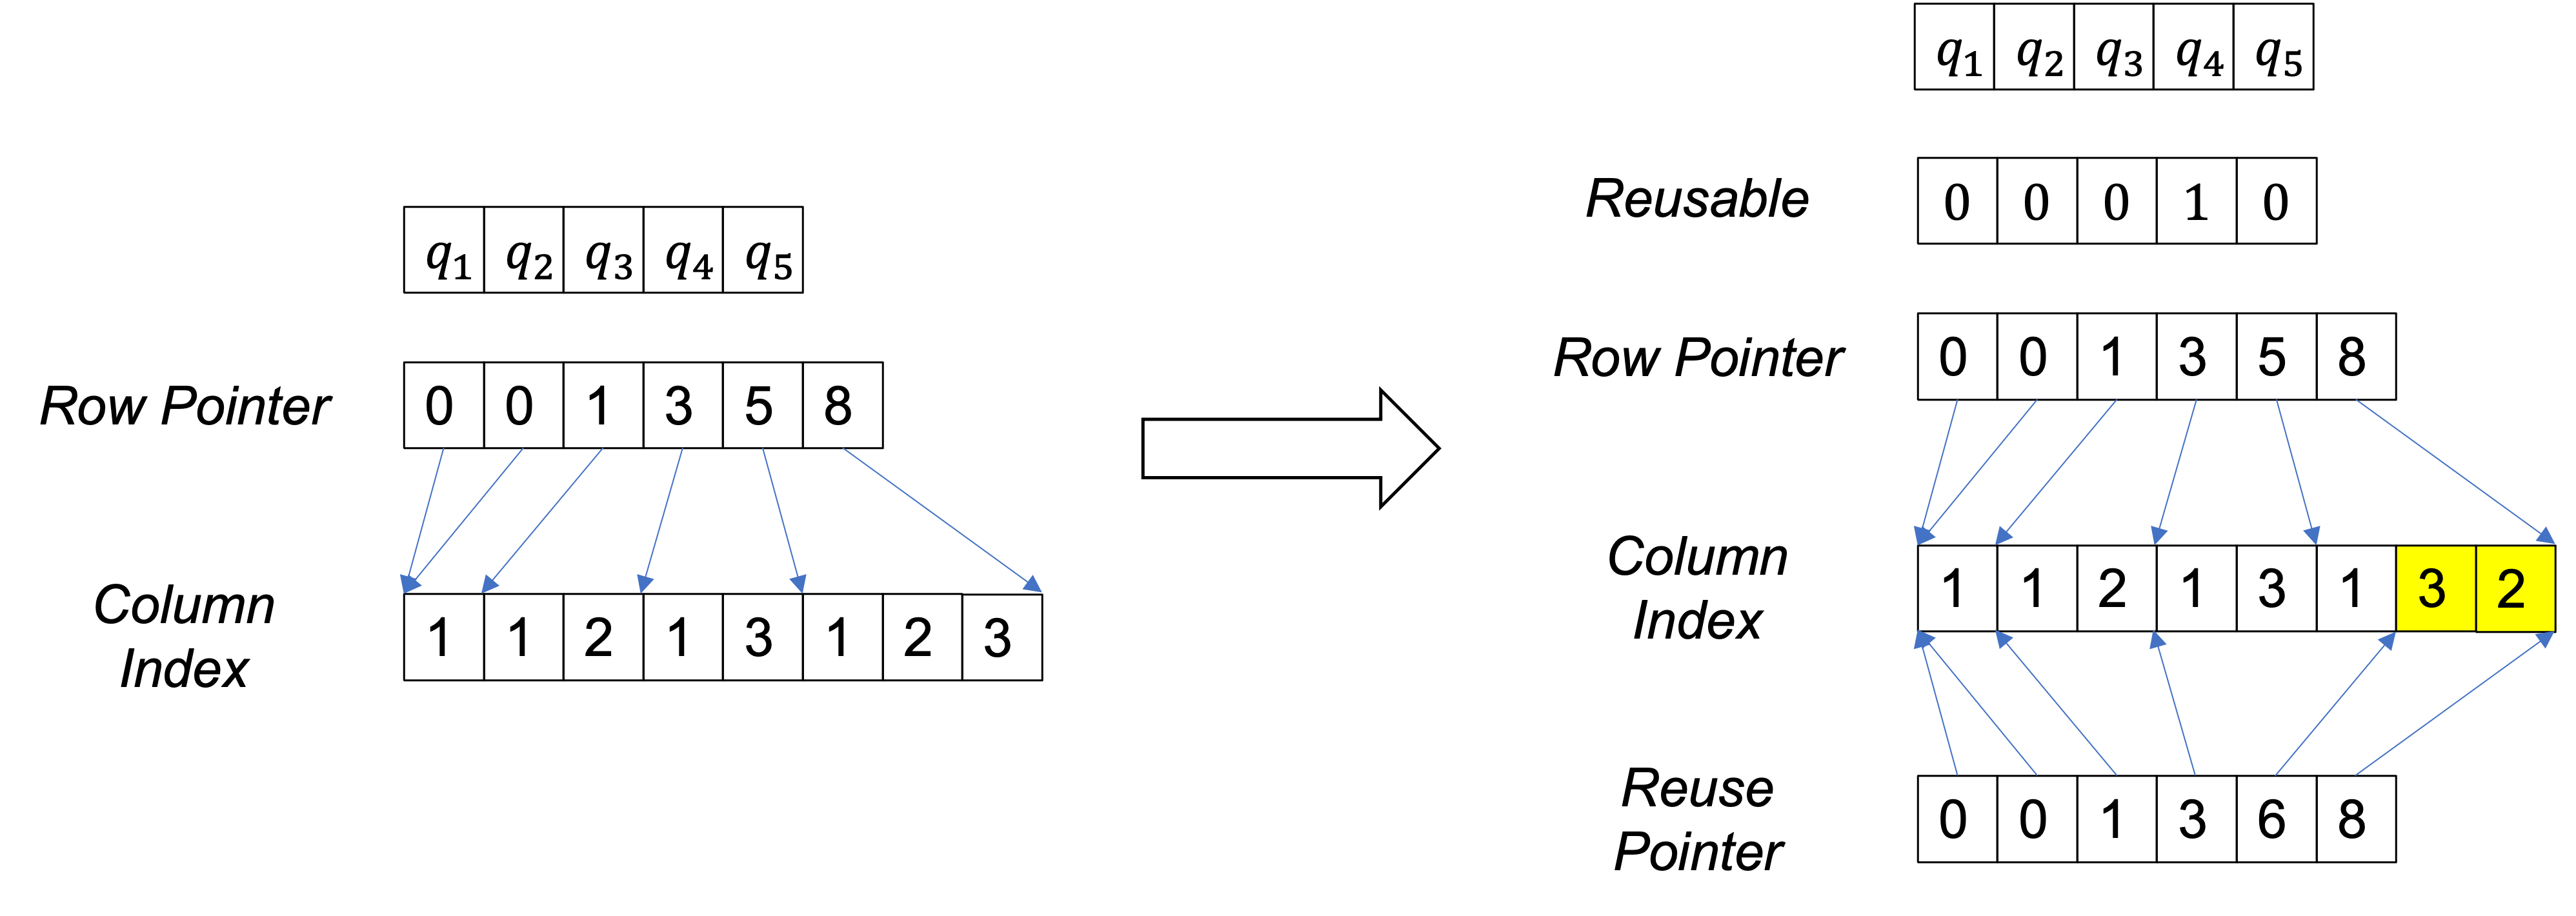
\includegraphics[width=\textwidth]{fig/improvements/Reuse-resorting.png}
    \caption{Reuse Detection Example}
    \label{fig:reuse-detection}
\end{figure}
Once the reuse is detected and pointers are set, the data is sent to the GPU constant memory for the rest of the application. For implementing reuse, the function in Algorithm \ref{algo:intersect} needs to be changed to add conditions for checking if a level is reusable or if the reuse pointer is updated.
These changes are shown as a flow chart in Figure \ref{fig:reuse-flowchart}.
\begin{figure}
    \centering
    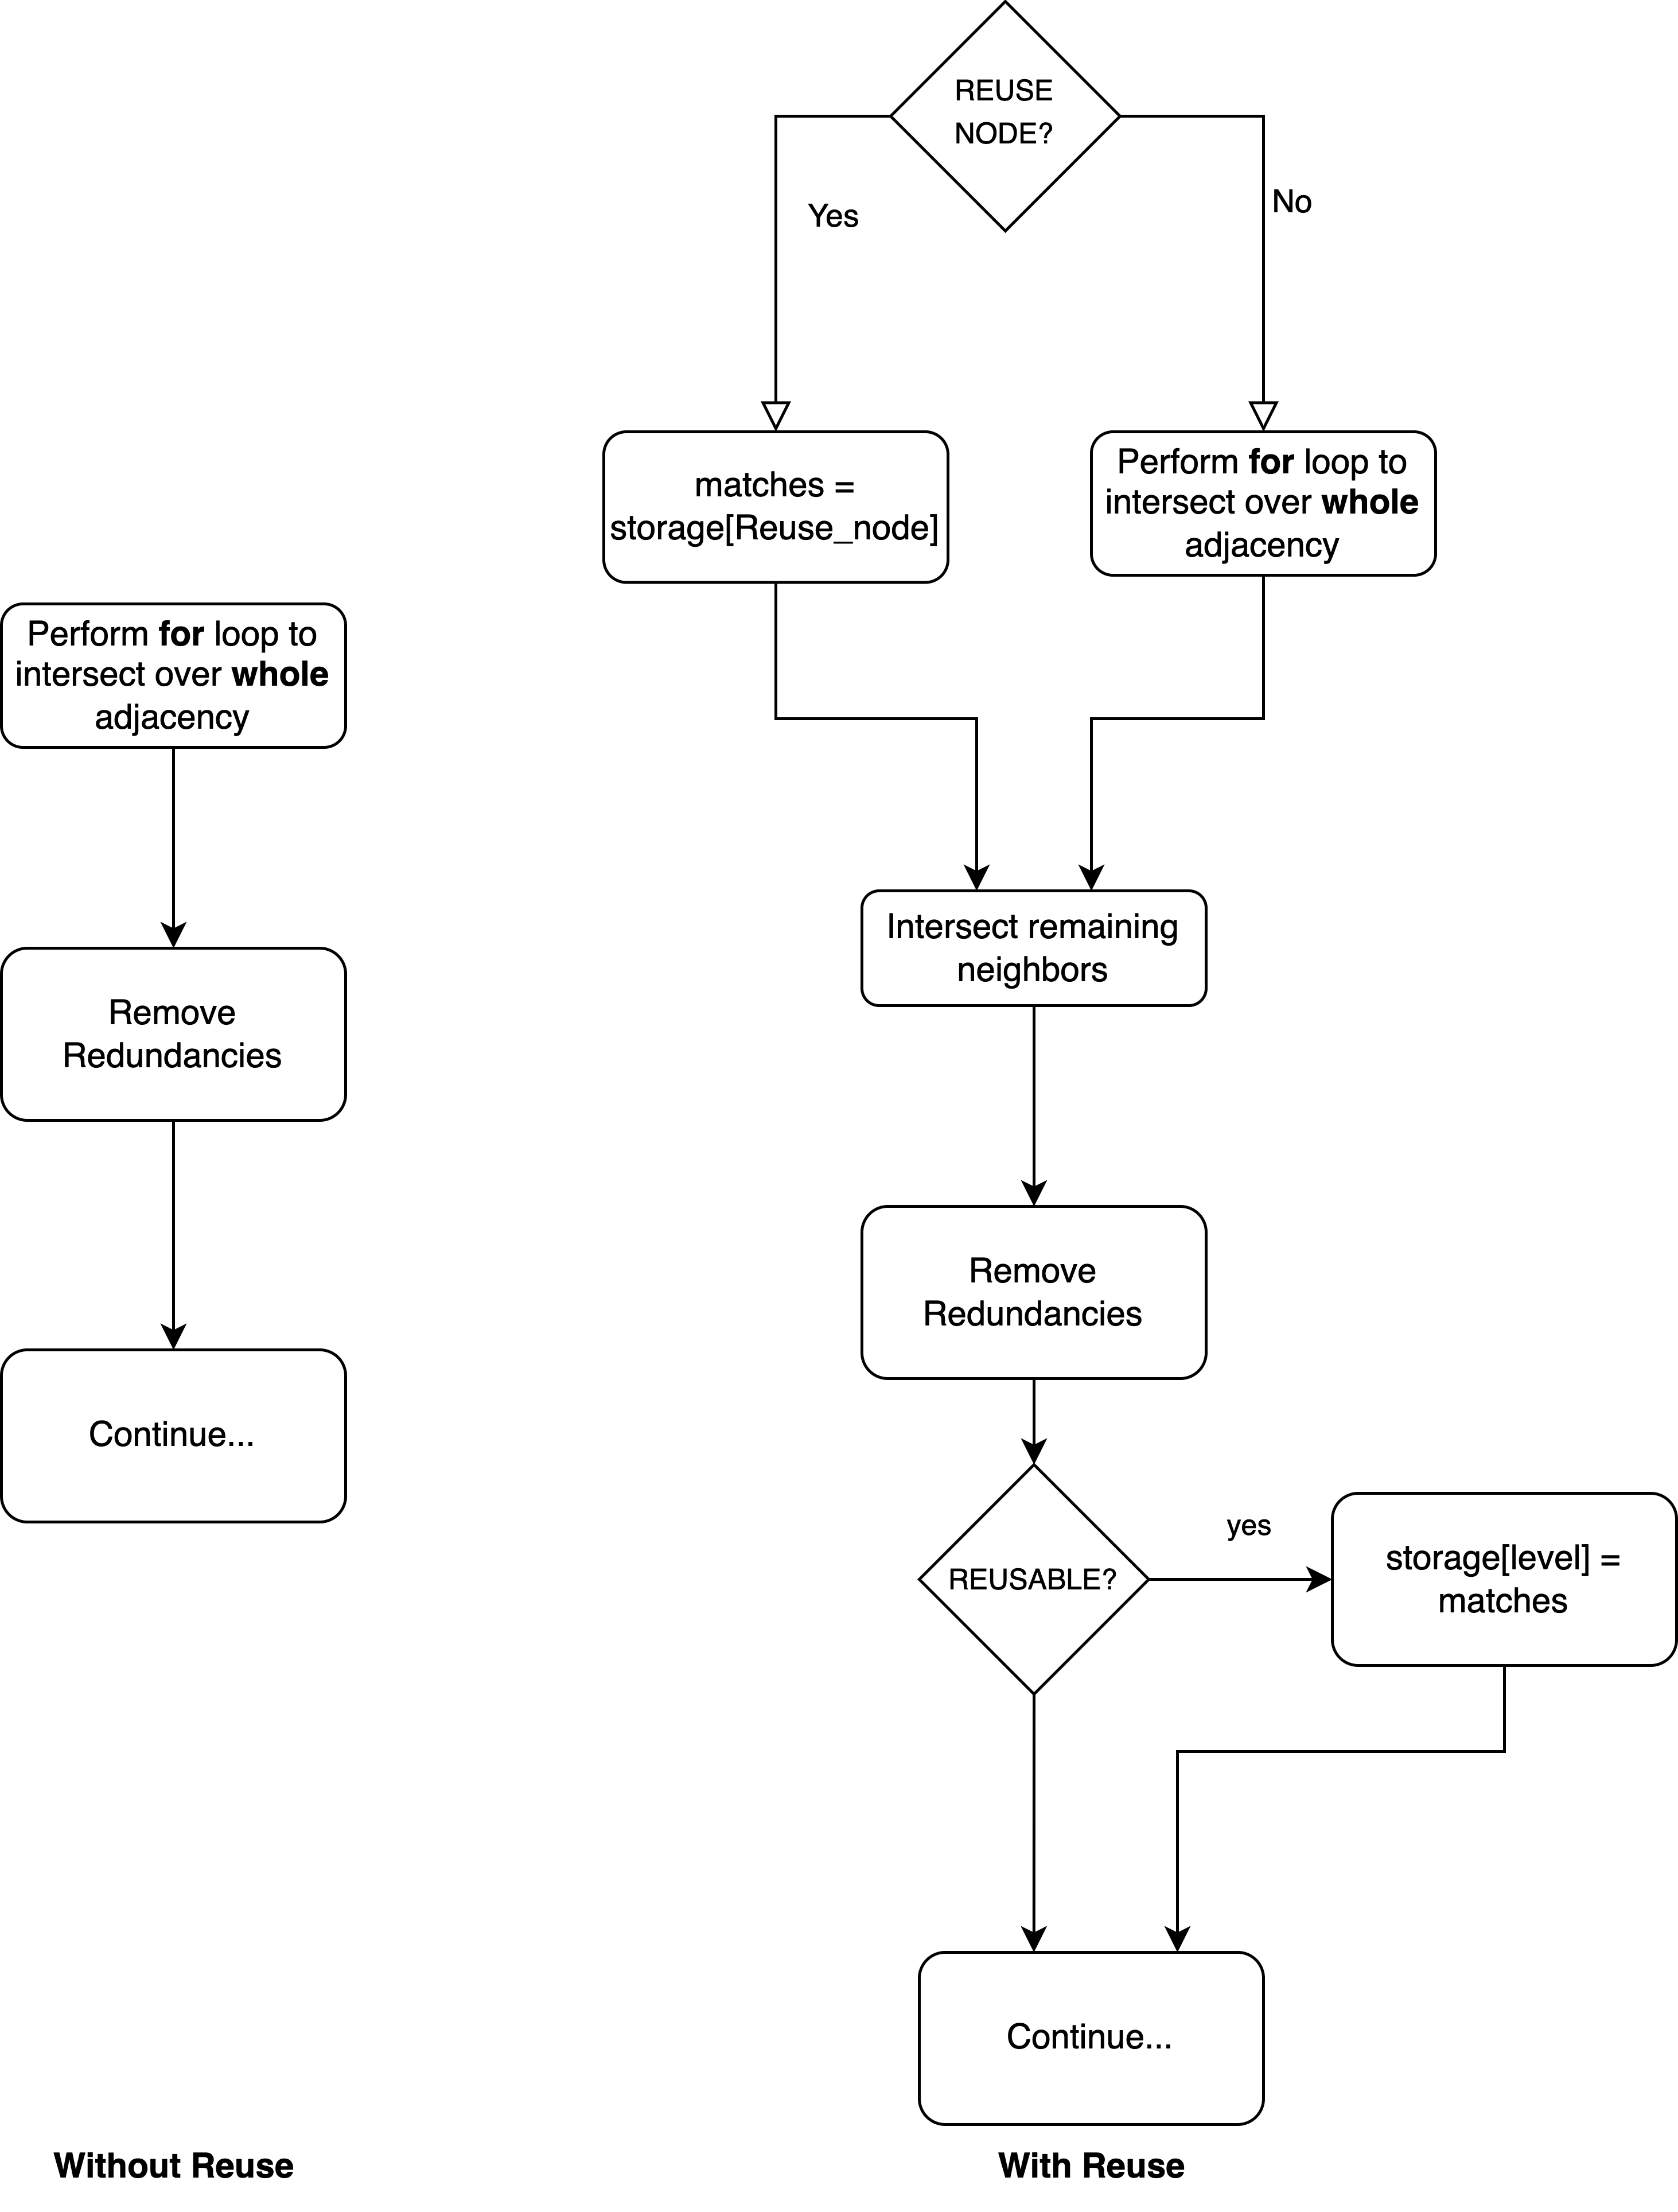
\includegraphics[width=\textwidth]{fig/improvements/reuse-flow1.png}
    \caption{Flowchart with and without reuse}
    \label{fig:reuse-flowchart}
\end{figure}
This way, reuse reduces computational workload and adds to the memory workload.
Since global memory writes are relatively expensive, some shared memory can be utilized to write the intermediate intersection results while longer results can be spilled to global memory.

\begin{algorithm}
    \caption{Reuse Detection}
    \label{algo:reuse}
    \SetKwData{qgraph}{$G_q=(V_q, E_q)$}
    \SetKwData{bneighbor}{$\mathcal{N}(V_q)$}
    \SetKwData{reusable}{$\texttt{reusable}$}
    \KwIn{Directed Query Graph \qgraph \newline
        Arrray of Backward Neighbor lists \bneighbor
    }
    $W \leftarrow: [|V_q|][|V_q|]$\;
    $X \leftarrow: [|V_q|][|V_q|]$\;
    \reusable $\leftarrow: [|V_q|]$\;
    \ForAll{$j \in V_q$}{
        \For{$i=j+1 \textbf{ to } |V_q|$}{
            \leIf{$\bneighbor[i] \supseteq \bneighbor[j]$}{
                $W[i][j] \leftarrow |\bneighbor[i] \cap \bneighbor[j]|$\;
            }
            {
                $W[i][j] \leftarrow 0$
            }
        }
    }
    $\reusable[j] \leftarrow (\max({W[i].)} > 0)$\;
    \ForAll{$i \in V_q$}{
        \For{$j=1 \textbf{ to } i$}{
            \leIf(){$j==\argmax_j(W[i]. > 0)$}{$1$\; $\reusable[j]=1$\;}{0}
        }
    }
    \CommentSty{\texttt{// Update Reuse Pointers from $X[i][j]$}}
\end{algorithm}

The improvements due to intersection reuse are measured using intersection speedup.
Since there are increased memory accesses and additional \textit{if-else} conditions, the time benefit from this technique is negligible. Table \ref{tab:reuse-improvement} shows the improvement in the number of intersections with this technique.
The intersection counts reported here also include additional read and write operations required by intersection reuse.
Since the backward neighbors lists are small for sparse queries, the benefits due to intersection reuse are limited.

\begin{table}[tbp]
    \centering
    \caption{Number of intersections with and without reuse for com-youtube}
    % \resizebox{\textwidth}{!}{%
    \begin{tabular}{c|rrc}
        \hline
        Query                                                                  & \begin{tabular}[r]{@{}r@{}}\#Intersections  \\w/o Reuse  \end{tabular} &
        \begin{tabular}[r]{@{}r@{}} \#Intersections \\with Reuse \end{tabular} &
        \begin{tabular}[r]{@{}r@{}} Intersection \\Speedup     \end{tabular}                                                                                                 \\ \hline
        diamond                                                                & 9,722,143                                                              & 9,722,143   & 1.00 \\
        cq4                                                                    & 6,028,832                                                              & 6,028,832   & 1.00 \\
        cq5\_m1                                                                & 46,794,486                                                             & 26,360,303  & 1.78 \\
        cq5                                                                    & 20,881,838                                                             & 15,889,824  & 1.31 \\
        cq6\_m1                                                                & 130,114,516                                                            & 52,225,436  & 2.49 \\
        cq6                                                                    & 49,618,729                                                             & 30,194,042  & 1.64 \\
        cq7\_m1                                                                & 253,215,589                                                            & 81,007,445  & 3.13 \\
        cq7                                                                    & 91,679,280                                                             & 46,935,236  & 1.95 \\
        cq8\_m1                                                                & 370,669,539                                                            & 102,639,103 & 3.61 \\
        cq8                                                                    & 139,279,024                                                            & 62,709,660  & 2.22 \\
        cq9\_m1                                                                & 430,334,955                                                            & 111,122,133 & 3.87 \\
        cq9                                                                    & 181,479,780                                                            & 74,663,152  & 2.43 \\
    \end{tabular}%
    % }
    \label{tab:reuse-improvement}
\end{table}

\section{Hybrid Symmetry Breaking}\label{sec:hy-symbreak}
Symmetry breaking is an important operation in the search tree traversal.
\cite{ullman_sgm} gives a simple ordering technique for symmetry breaking, but the ordering criteria are not well-defined.
Any criterion can be used for correctness, but efficient criteria can significantly improve performance due to slimmer search tree.
Handling symmetries to reduce the search space is an active area of research.
The problem of finding an efficient symmetry breaking criteria was shown to be strongly NP-hard by \cite{crawford-sb-np-hard}.
A lot of symmetry breaking criteria have been defined since then.
However, most of them have linear time complexity or need BFS traversal.
In the optimization domain, this problem has also been formulated as a Constraint Satisfaction Problem (CSP) but it also works only when the tree traversal is done in BFS fashion \cite{sb-CSP}.
The near-linear time complexity for each decision, constraints to perform BFS, and data sharing between subtrees make efficient symmetry breaking difficult on GPUs.
To avert these, we resort to static characteristics like Degree and Degeneracy.
The structure generated due to priority sorted column index array (PSCI) (discussed in Section \ref{sec:prio-sorting}) is used to further reduce global memory accesses.

With PSCI, different symmetry breaking criteria were tried and compared to the baseline \cite{PARSEC_VD}.
The baseline criteria are based on degree for level 1 and lexicographic for level 2 onwards.
The symmetry breaking performance is determined by intersection speedup.
On performing these experiments, the degeneracy-based symmetry breaking seemed to perform worse than baseline across all graphs.
For degree, run  degree-based criterion seemed to perform better for some queries while decreasing criterion performed better for others.
Table \ref{tab:degree-sb} shows the intersection speedups for \textit{soc-pokec} and \textit{cit-patents} data graphs.
% On further analysis it was found that the templates for which decreasing ordering works better mostly had second-level asymmetric to first.

\begin{table}[h]
    \centering
    \caption{Intersection Speedup with Degree based Symmetry Breaking}

    \resizebox{\textwidth}{!}{
        \begin{tabular}{r|cccccccccc}
            \hline
            \textbf{soc-pokec}   &
            Tri                  &
            Diamond              &
            Cq4                  &
            Cq5m1                &
            Cq5                  &
            House                &
            Pyramid              &
            Fan3                 &
            Cq6m1                &
            Cq6                                                                                                 \\\hline
            \textbf{Decreasing}  &
            1.22                 &
            0.53                 &
            0.66                 &
            0.89                 &
            1.19                 &
            1.49                 &
            1.88                 &
            1.76                 &
            1.06                 &
            1.41                                                                                                \\
            \textbf{Increasing}  &
            3.00                 &
            1.08                 &
            1.47                 &
            1.67                 &
            2.29                 &
            2.85                 &
            0.22                 &
            0.20                 &
            1.64                 &
            2.25                                                                                                \\
            \\
            \hline
            \textbf{cit-patents} & Tri  & Diamond & cq4  & cq5m1 & cq5  & house & pyramid & fan3 & cq6m1 & cq6  \\\hline
            \textbf{Decreasing}  & 1.22 & 0.82    & 1.24 & 2.32  & 2.91 & 4.29  & 3.15    & 3.92 & 2.51  & 3.15 \\
            \textbf{Increasing}  & 3.00 & 1.27    & 1.79 & 3.50  & 4.28 & 6.60  & 1.26    & 1.83 & 2.72  & 3.71
        \end{tabular}
    }
    \label{tab:degree-sb}
\end{table}


Recall from \ref{sec:sym-detection} that the symmetry breaking criteria can be different for different levels and maybe different for different subtrees.
% To precisely find out when it can be different and when it cannot, we present the following observation:
We present the following observation to precisely find out when the criteria can be different across subtrees.
\begin{theorem} \label{thm:hybrid-sb}
    Symmetry breaking is independent across subtrees for central node queries with first symmetric level greater than two.
\end{theorem}
\begin{proof}
    Let, the data graph be $G=(V, E)$ and $\{v_1, v_2\} \in V$.\\
    $G_{ind}(v)$ be the subgraph induced by $v$ in $G$.\\
    The backward neighbors list of a vertex is represented by $\mathcal{N}'(.)$.\\
    % Trivial if $) = \phi $
    Consider $X:=\mathcal{E}(G_{ind}(v_1)) \cap \mathcal{E}(G_{ind}(v_2)$\\
    % The proof is non trivial only if $X \neq \phi$.\\
    Assume, $X$ to be non-empty. (proof is trivial otherwise)\\
    $ \forall ~ \text{edges }(x,y) \in X$:
    Since, $(x,y) \in \mathcal{E}(G_{ind}(v_1)) ~ \Rightarrow ~ x,y \in \mathcal{N}(v_1)$\\
    Similarly,  $x,y \in \mathcal{N}(v_2)$

    Now for Algorithm \ref{algo:DFS-traversal}, since level 2 vertex (say $q_2$) in the query graph is not symmetric to the level 1 vertex (say $q_1$), candidates for level 2 will be given by adjacency list intersections of matches in $\mathcal{N'}(q_2)$.

    Since, $q_1$ has to be a central node, $\mathcal{N'}(q_2)=q_1 \Rightarrow $ level 2 candidates for tree rooted at $v_1$ will be $\mathcal{N}(v_1)$ and for tree rooted at $v_2$ they will be $\mathcal{N}(v_2).$
    Therefore, all edges in $X$ are added to both search trees.\\
    This implies, each subtree will enumerate the correct number of query instances independent of the symmetry breaking strategy.
\end{proof}

Theorem \ref{thm:hybrid-sb} enables individual symmetry breaking criteria for subtrees.
Table \ref{tab:degree-sb} shows the best strategy depends on the data graph as well as query graph.
The optimal strategy may even be different for distinct subtrees in the same data graph.

To curb the variability in strategy decisions, a dynamic two-phase traversal technique is designed:
The first phase is to determine if a particular subtree should perform increasing or decreasing symmetry breaking.
The second phase is to use the predetermined strategy to execute the search tree traversal.
% Performing increasing or decreasing symmetry breaking differs by one step hence the second phase can simply check the predetermined strategy and prune accordingly.

For the first phase, since the problem of finding an optimal symmetry breaking criterion is strongly NP-hard, any practical implementation can only develop Heuristics.
A natural strategy to decide the criteria in phase one might seem to be based on counting the number of eligible candidates till the first symmetric level.
This approach does not always work as both strategies might produce equal number of candidates at the first symmetric level.
Also, fewer candidates at first symmetric level does not necessarily reflect in a smaller search tree.
% This hints that there should be a criterion to determine the \textit{quality} of these candidates.
This hints at designing a criterion to determine the \textit{quality} of these candidates.
Since the candidates generated are sorted by priority, we use the following observations to determine their \textit{quality}:
\begin{enumerate}[1.]
    \item For increasing symmetry breaking, the left side of the DFS subtree has fewer candidates (vice versa for decreasing).
    \item Few candidates on the left side may generate more nodes in subsequent levels, while the right side candidates (high count) might not.
\end{enumerate}
So the weights should be selected based on an equalizing philosophy where higher weight is given to the left side of the tree (for increasing symmetry breaking).
Increasing weights based on the index of candidates and the total number of candidates is used for this purpose.

To formalize, Let the total number of candidates at $j^{th}$ leaf in the subtree be $C_j$ and the number of candidates found  in the previous level be $S$.
The symmetry breaking criterion is determined based on the weighted sum ($WS$).
$$WS = \sum_j C_j\times W_j$$
The weightage $W_j$ for the quality of this branch is given by:
$$
    W_j=\begin{cases}
        (S - j) \text{ for increasing and,} \\
        j \text{ for decreasing}.
    \end{cases}
$$
A criterion is picked for the subtree based on whichever weighted sum is smaller.

To find the efficiency of this strategy, we compare it with the best, worst, and pure strategies using intersection speedup.
Table \ref{tab:hybrid-symbreak-performance} shows that hybrid strategy often works better than pure strategies and is sometimes close to the best possible strategy.
% This improvement in reduced work reflects in time improvements.
Table \ref{tab:speedups-hy-sym} gives the time speedups for \textit{fan3} and \textit{pyramid} across different data graphs.
Note, these queries were specifically selected since their first symmetric level is greater than two.
% So the hybrid symmetry breaking does not rely on pure strategy.
The reasons for intersection speedups not proportionally reflecting in time speedups are time for other operations, load imbalance, and two-phase strategy overheads.

\begin{table}[]
    \centering
    \caption{Comparison of Hybrid strategy with pure, best and worst possible strategies using intersection speedup criteria for data graph cit-patents}
    % \resizebox{\textwidth}{!}{%
    \begin{tabular}{r|ccccc}
        \hline
        \textbf{Query} & \textbf{Increasing} & \textbf{Decreasing} & \textbf{Hybrid} & \textbf{Best} & \textbf{Worst} \\\hline
        Tri            & 3.00                & 2.20                & 3.00            & 3.00          & 2.20           \\
        Diamond        & 1.27                & 0.82                & 1.27            & 1.27          & 0.82           \\
        cq4            & 1.79                & 1.24                & 1.79            & 1.79          & 1.24           \\
        cq5m1          & 3.50                & 2.32                & 3.50            & 3.50          & 2.32           \\
        cq5            & 4.28                & 2.91                & 4.28            & 4.28          & 2.91           \\
        house          & 6.60                & 4.29                & 6.60            & 6.60          & 4.29           \\
        pyramid        & 1.26                & 2.45                & 2.47            & 2.53          & 1.24           \\
        fan3           & 1.83                & 3.92                & 3.96            & 4.07          & 1.80           \\
        cq6m1          & 2.72                & 2.51                & 2.72            & 2.72          & 2.51           \\
        wheel5         & 1.00                & 1.57                & 1.57            & 1.57          & 0.99           \\
        fan4           & 1.56                & 2.20                & 2.22            & 2.22          & 1.56           \\
        cq6            & 3.71                & 3.15                & 3.71            & 3.71          & 3.15           \\
    \end{tabular}%
    % }
    \label{tab:hybrid-symbreak-performance}
\end{table}


\begin{table}[]
    \centering
    \caption{Time speedups with hybrid Symmetry Breaking}
    \resizebox{\textwidth}{!}{%
        \begin{tabular}{r|cc|c|cc|c}
            \hline
            \multirow{4}{*}{\textbf{Data Graph}} & \multicolumn{6}{|c}{\textbf{Queries}}                                                                                                                                                                   \\ \hline
                                                 & \multicolumn{3}{|c|}{\textbf{Fan3}}     & \multicolumn{3}{|c}{\textbf{Pyramid}}                                                                                                                         \\ \cline{2-7}
                                                 & \multicolumn{2}{|c|}{\textbf{Time (s)}} & \multirow{2}{*}{\textbf{Speedup}}     & \multicolumn{2}{|c|}{\textbf{Time (s)}} & \multirow{2}{*}{\textbf{Speedup}}                                           \\
                                                 & \textbf{Baseline}                       & \textbf{Degree hybrid}                &                                         & \textbf{Baseline}                 & \textbf{Degree hybrid}                  \\ \hline
            \textbf{soc-pokec}                   & 2.464                                   & 1.500                                 & \textbf{1.643}                          & 3.086                             & 1.964                  & \textbf{1.571} \\
            \textbf{com-youtube}                 & 9.675                                   & 6.206                                 & \textbf{1.559}                          & 19.253                            & 10.335                 & \textbf{1.863} \\
            \textbf{cit-patents}                 & 0.534                                   & 0.425                                 & \textbf{1.256}                          & 0.598                             & 0.472                  & \textbf{1.265} \\
            \textbf{com-orkut}                   & 447.532                                 & 342.183                               & \textbf{1.308}                          & 996.422                           & 582.864                & \textbf{1.710} \\
            \textbf{as-skitter}                  & 60.851                                  & 40.456                                & \textbf{1.504}                          & 159.289                           & 84.530                 & \textbf{1.884}
        \end{tabular}%
    }
    \label{tab:speedups-hy-sym}
\end{table}


\section{Hybrid Parallelism for load balance}

As mentioned in Section \ref{sec:block-scheduling} load balance is an important criterion while designing parallelization schemes.
The baseline implementation \cite{PARSEC_VD} offered two types of parallelism \textit{node per block} and \textit{edge per block}.
Figure \ref{fig:parallelization-schemes} shows the difference between these parallelization schemes.
\begin{figure}
    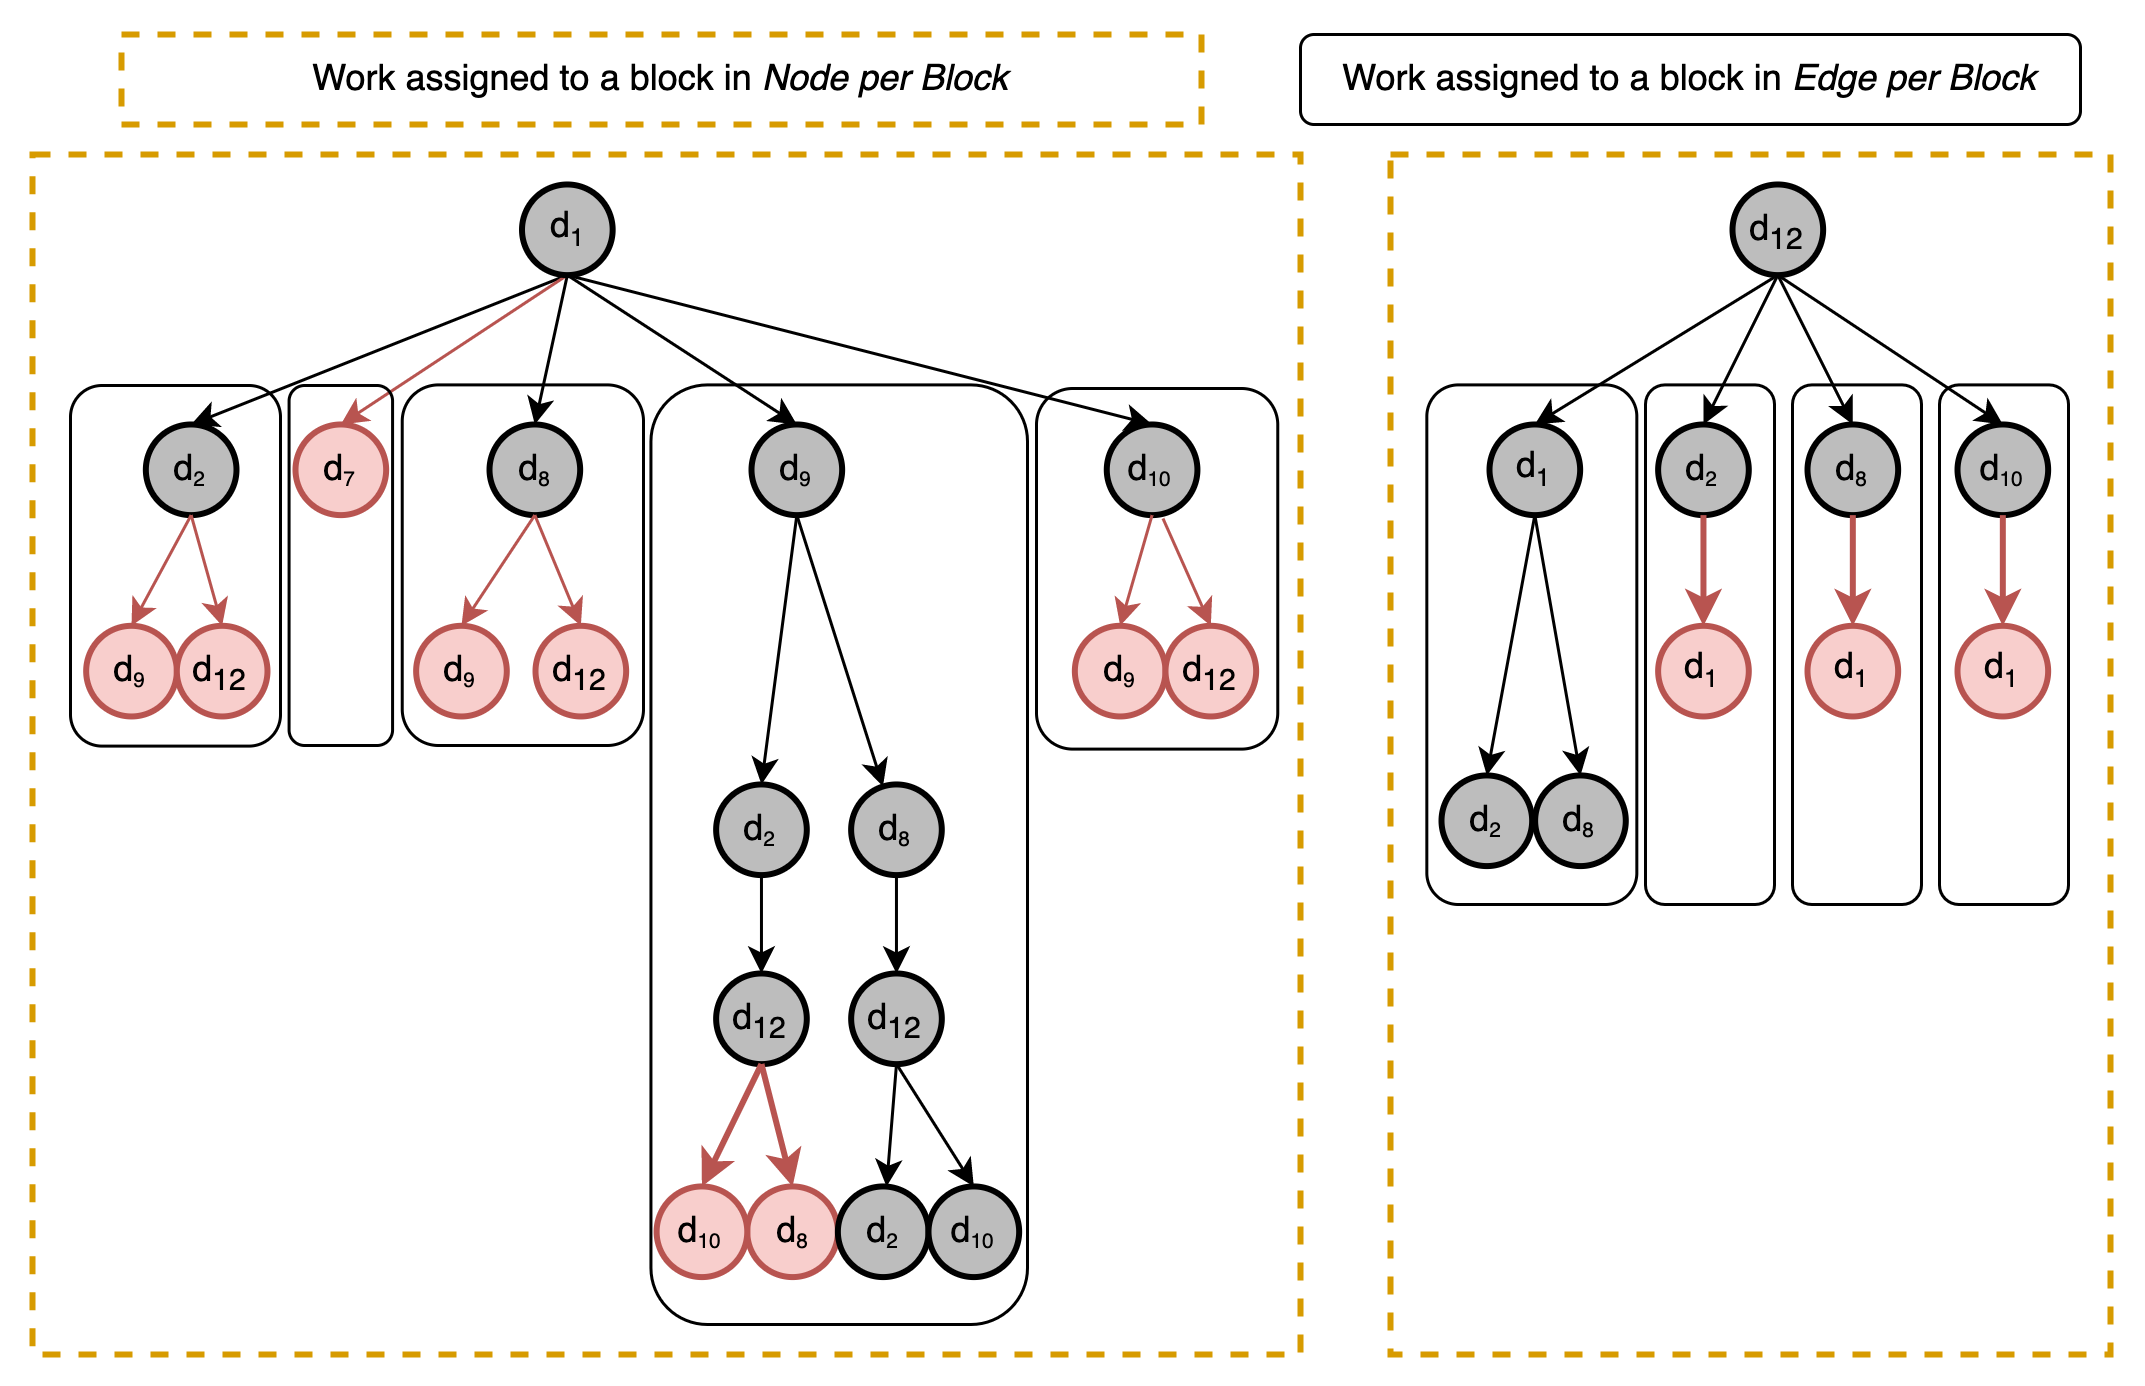
\includegraphics[width=\textwidth]{fig/parallelization-scheme.png}
    \caption{Parallelization Schemes}
    \label{fig:parallelization-schemes}
\end{figure}
% Two techniques were implemented to reduce the load imbalance, (1) Task scheduling, and (2) Hybrid Parallelism.
A hybrid parallelism technique was implemented to reduce the load balance.
Some insights from the baseline are presented for better understanding of this technique.
% , these insights also quantify the observations from baseline.
\subsubsection*{Observation 1 - Run time vs Degree}
Figure \ref{fig:run-time-vs-degree} shows the relationship between degree of the root node and run time as a log-log plot.
It is clear that run time is exponentially related to the root node degree. Moreover, there is huge variation in run time at the same degree.
\begin{figure}
    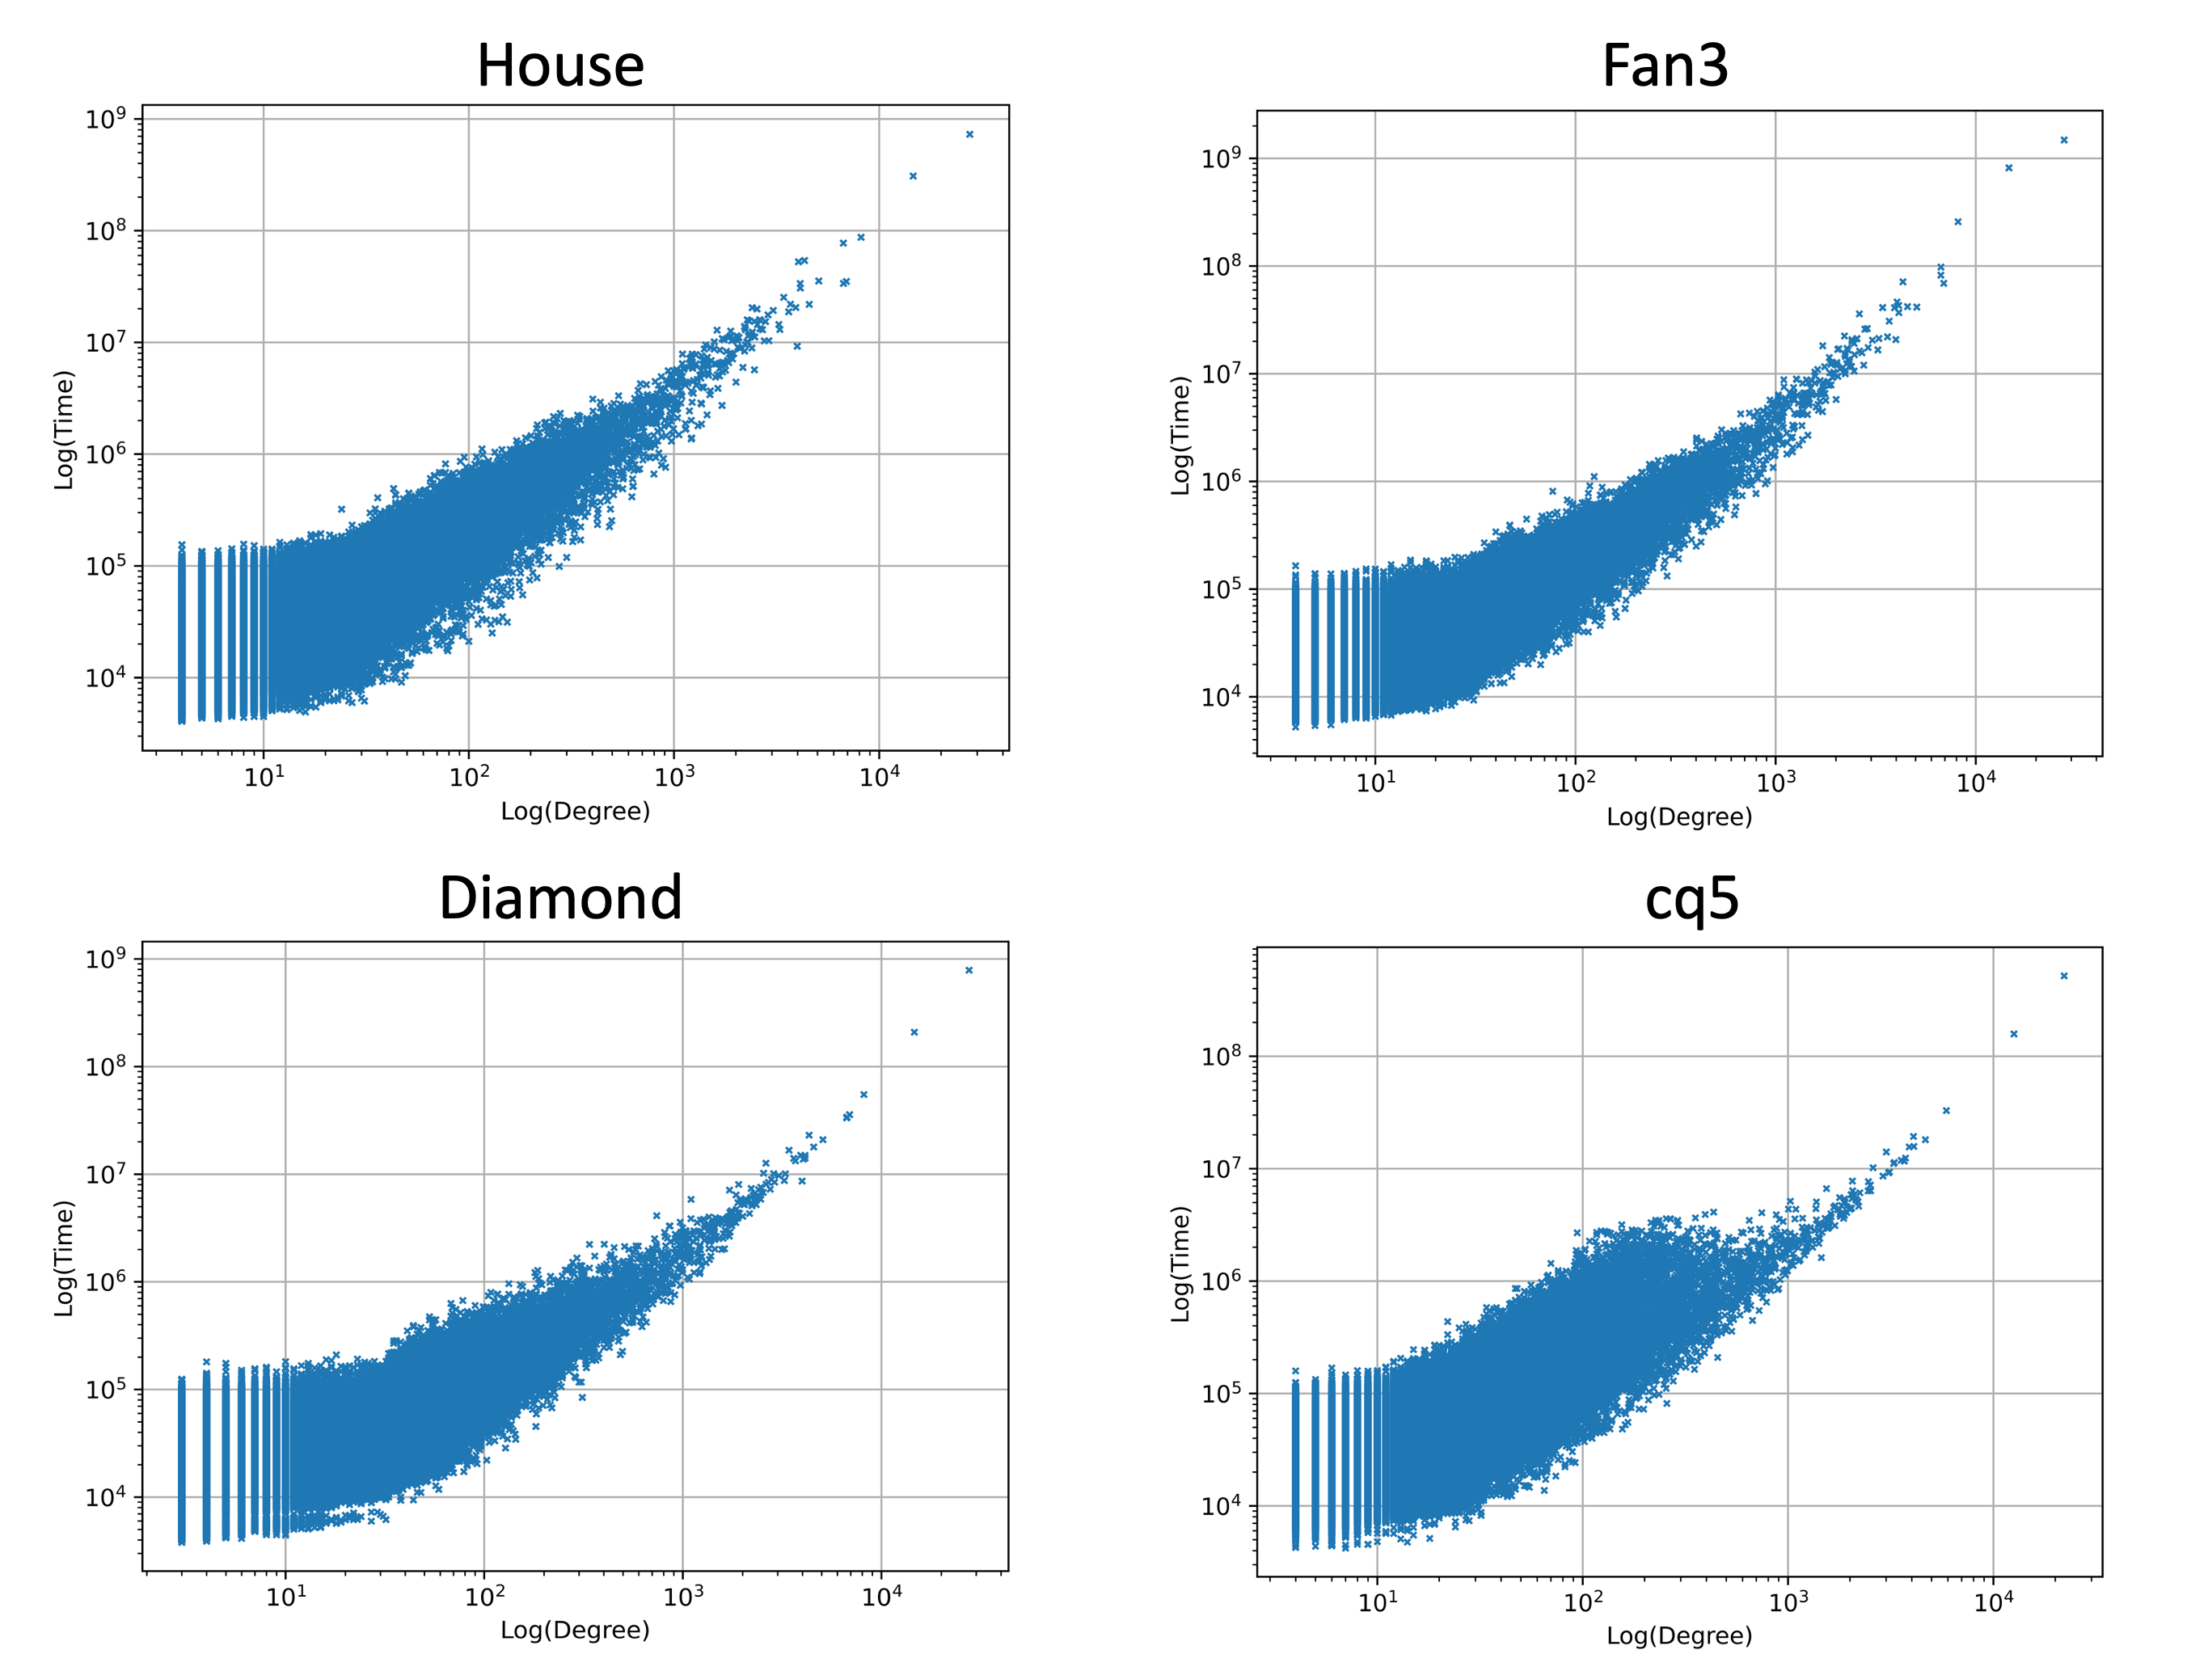
\includegraphics[width=\textwidth]{fig/improvements/time-vs-degree.png}
    \caption{Degree vs Run time for data graph com-youtube}
    \label{fig:run-time-vs-degree}
\end{figure}

\subsubsection*{Observation 2 - Load balance comparison}
Given the trend between run time and root node degree, the node per block scheme is expected to show a huge load imbalance.
The load balance is supposed to improve for the edge per block scheme as it would split the work offered by a high degree root node into several blocks.
Figure \ref{fig:load-balance-baseline} shows the load balance across SMs for various query graphs as a standard box plot.
This is computed by finding the relative processing time spent by each SM during kernel lifetime.
It is clear from the figure that the edge per block parallelization scheme significantly improves load balance.
\begin{figure}[t]
    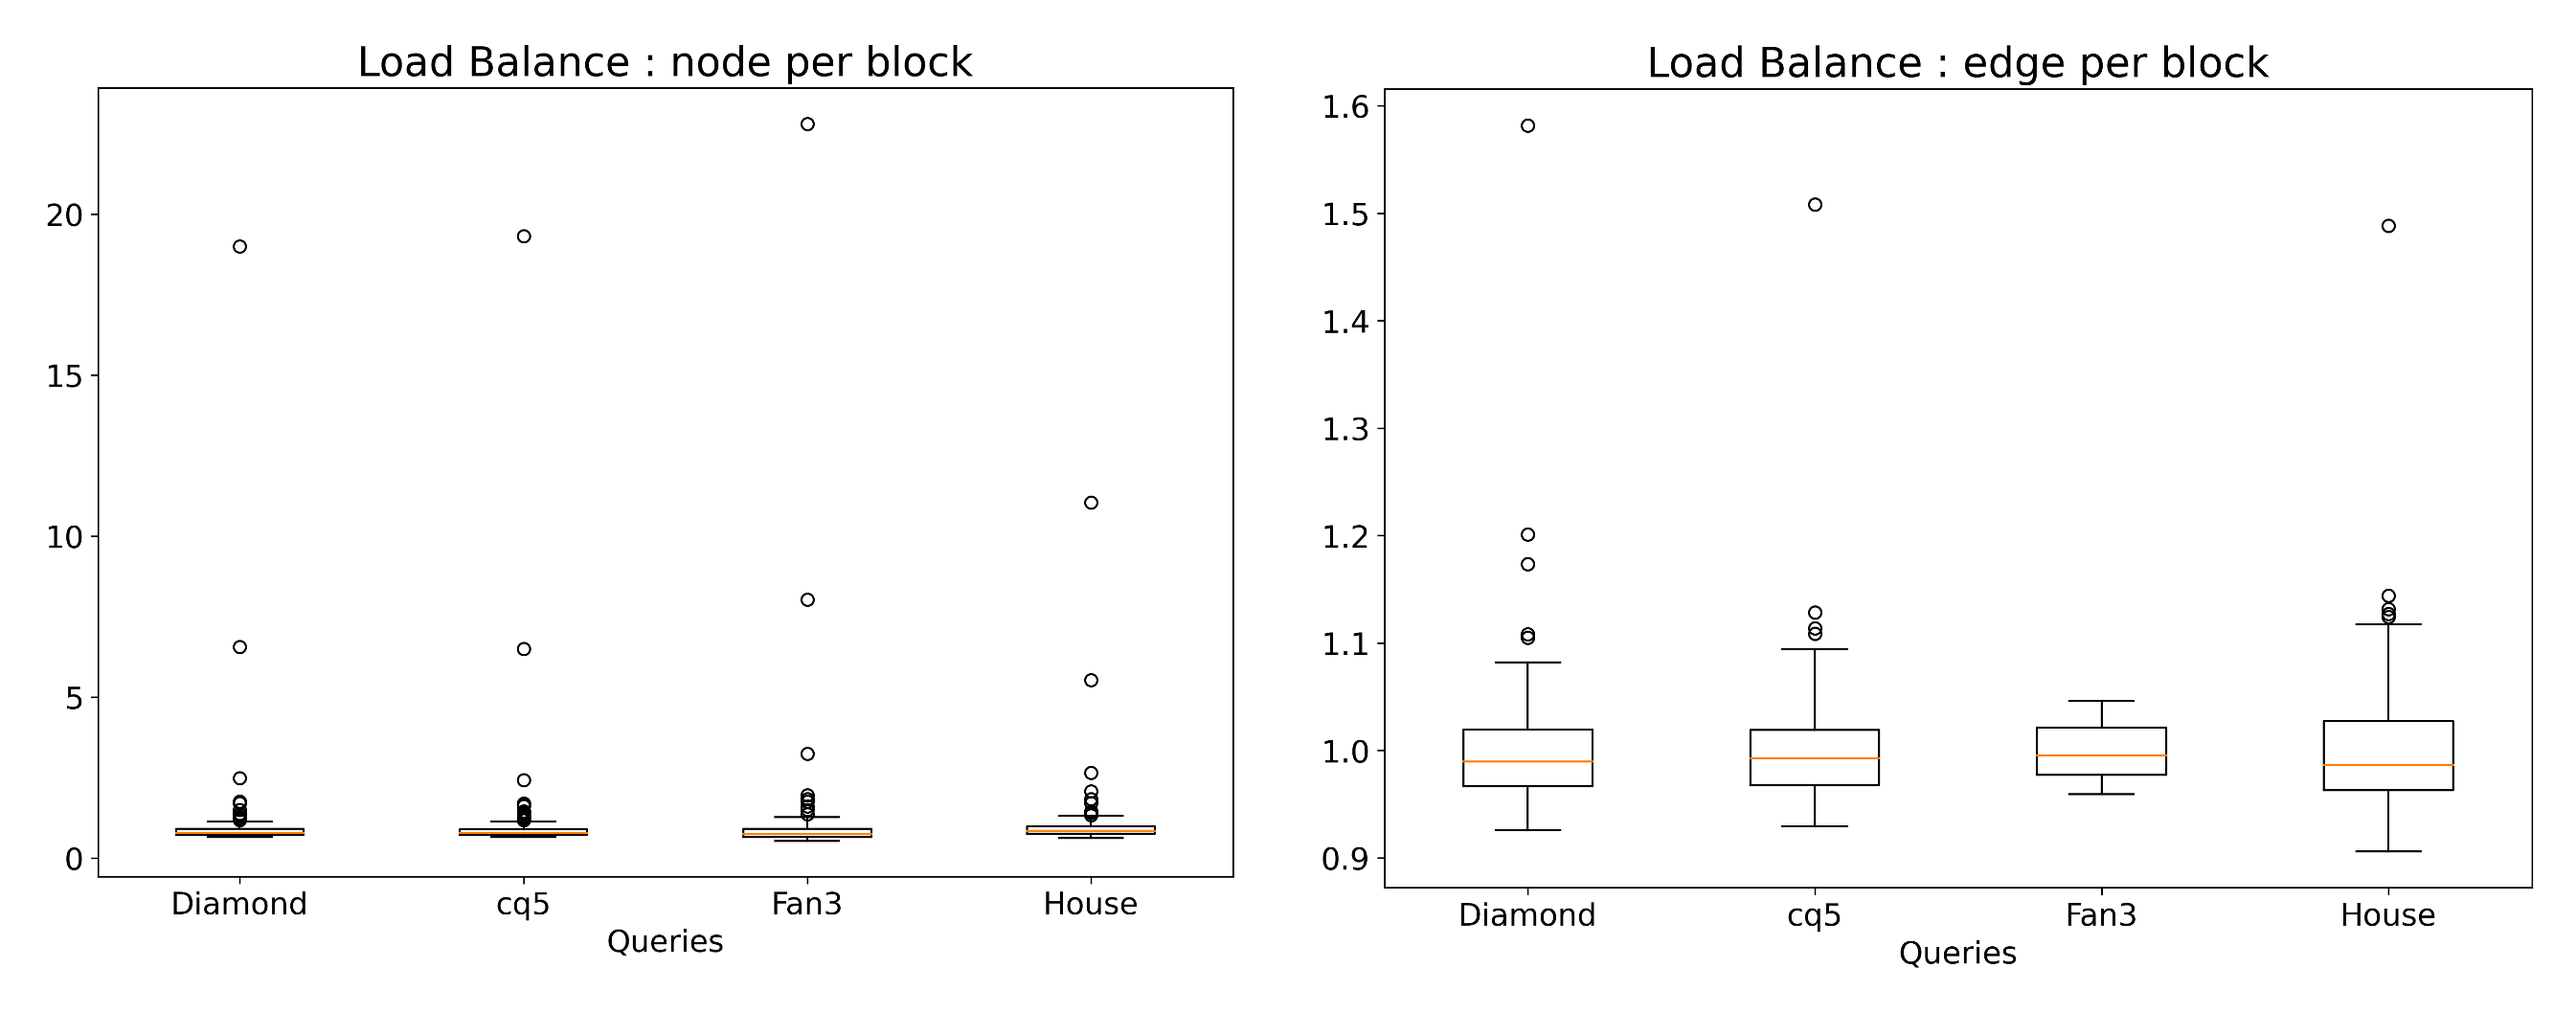
\includegraphics[width=\textwidth]{fig/improvements/yt_lb-baseline_byedge.png}
    \caption{com-youtube load balance with different parallelization schemes}
    \label{fig:load-balance-baseline}

    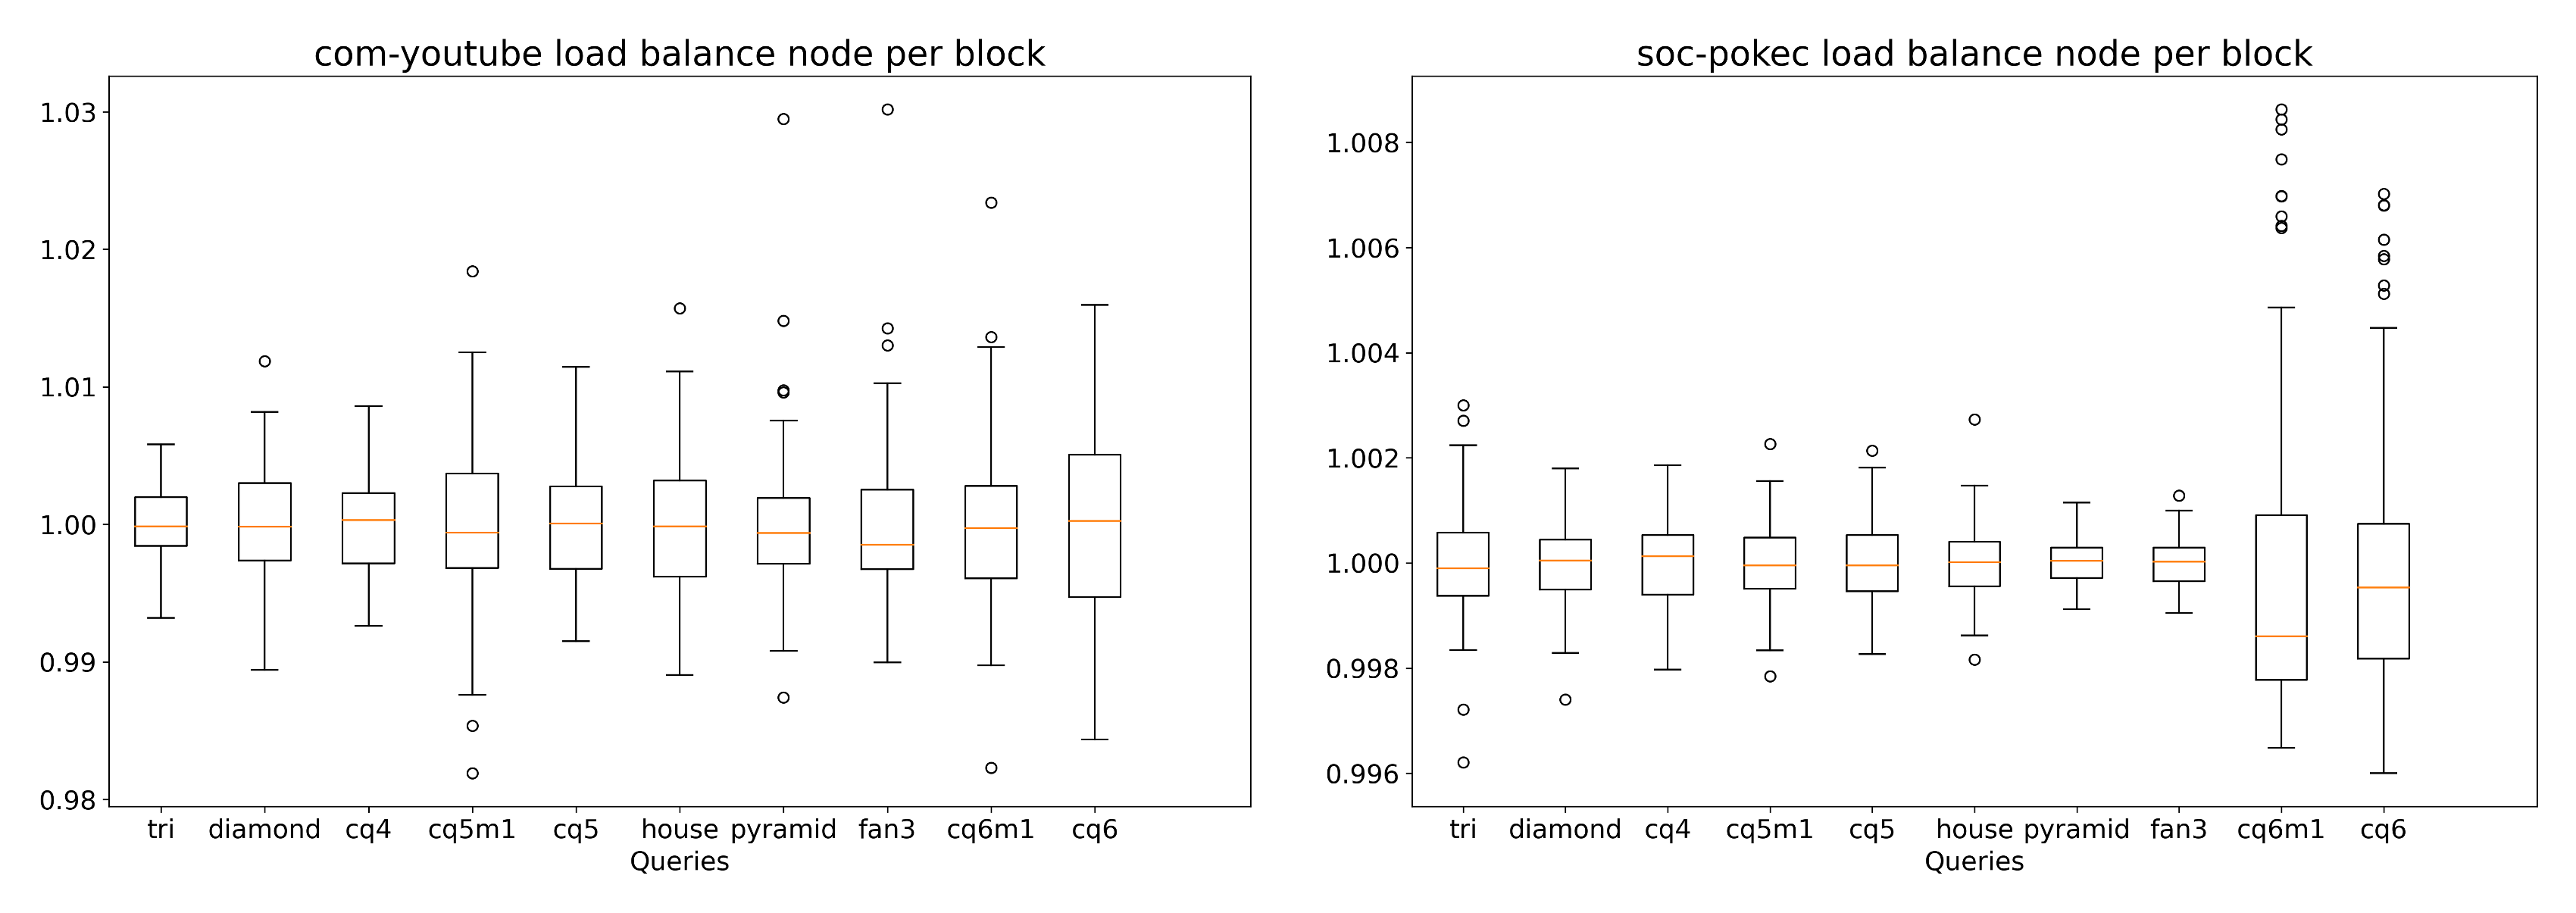
\includegraphics[width=\textwidth]{fig/improvements/load-balance-LD.png}
    \caption{Load balance for nodes with degree $\leq 256$ }
    \label{fig:load-balance-LD}
\end{figure}

\subsubsection*{Observation 3 - Load balance for low degree nodes}
Since the trend between degree and run time is exponential, the subtrees originating from nodes with low degrees will likely have lesser variation in run times.
Figure \ref{fig:load-balance-LD} shows there is negligible load imbalance when processing low degree nodes.
% For these findings, all nodes with degree higher than cutoff were filtered out before kernel launch.
% \begin{figure}
%     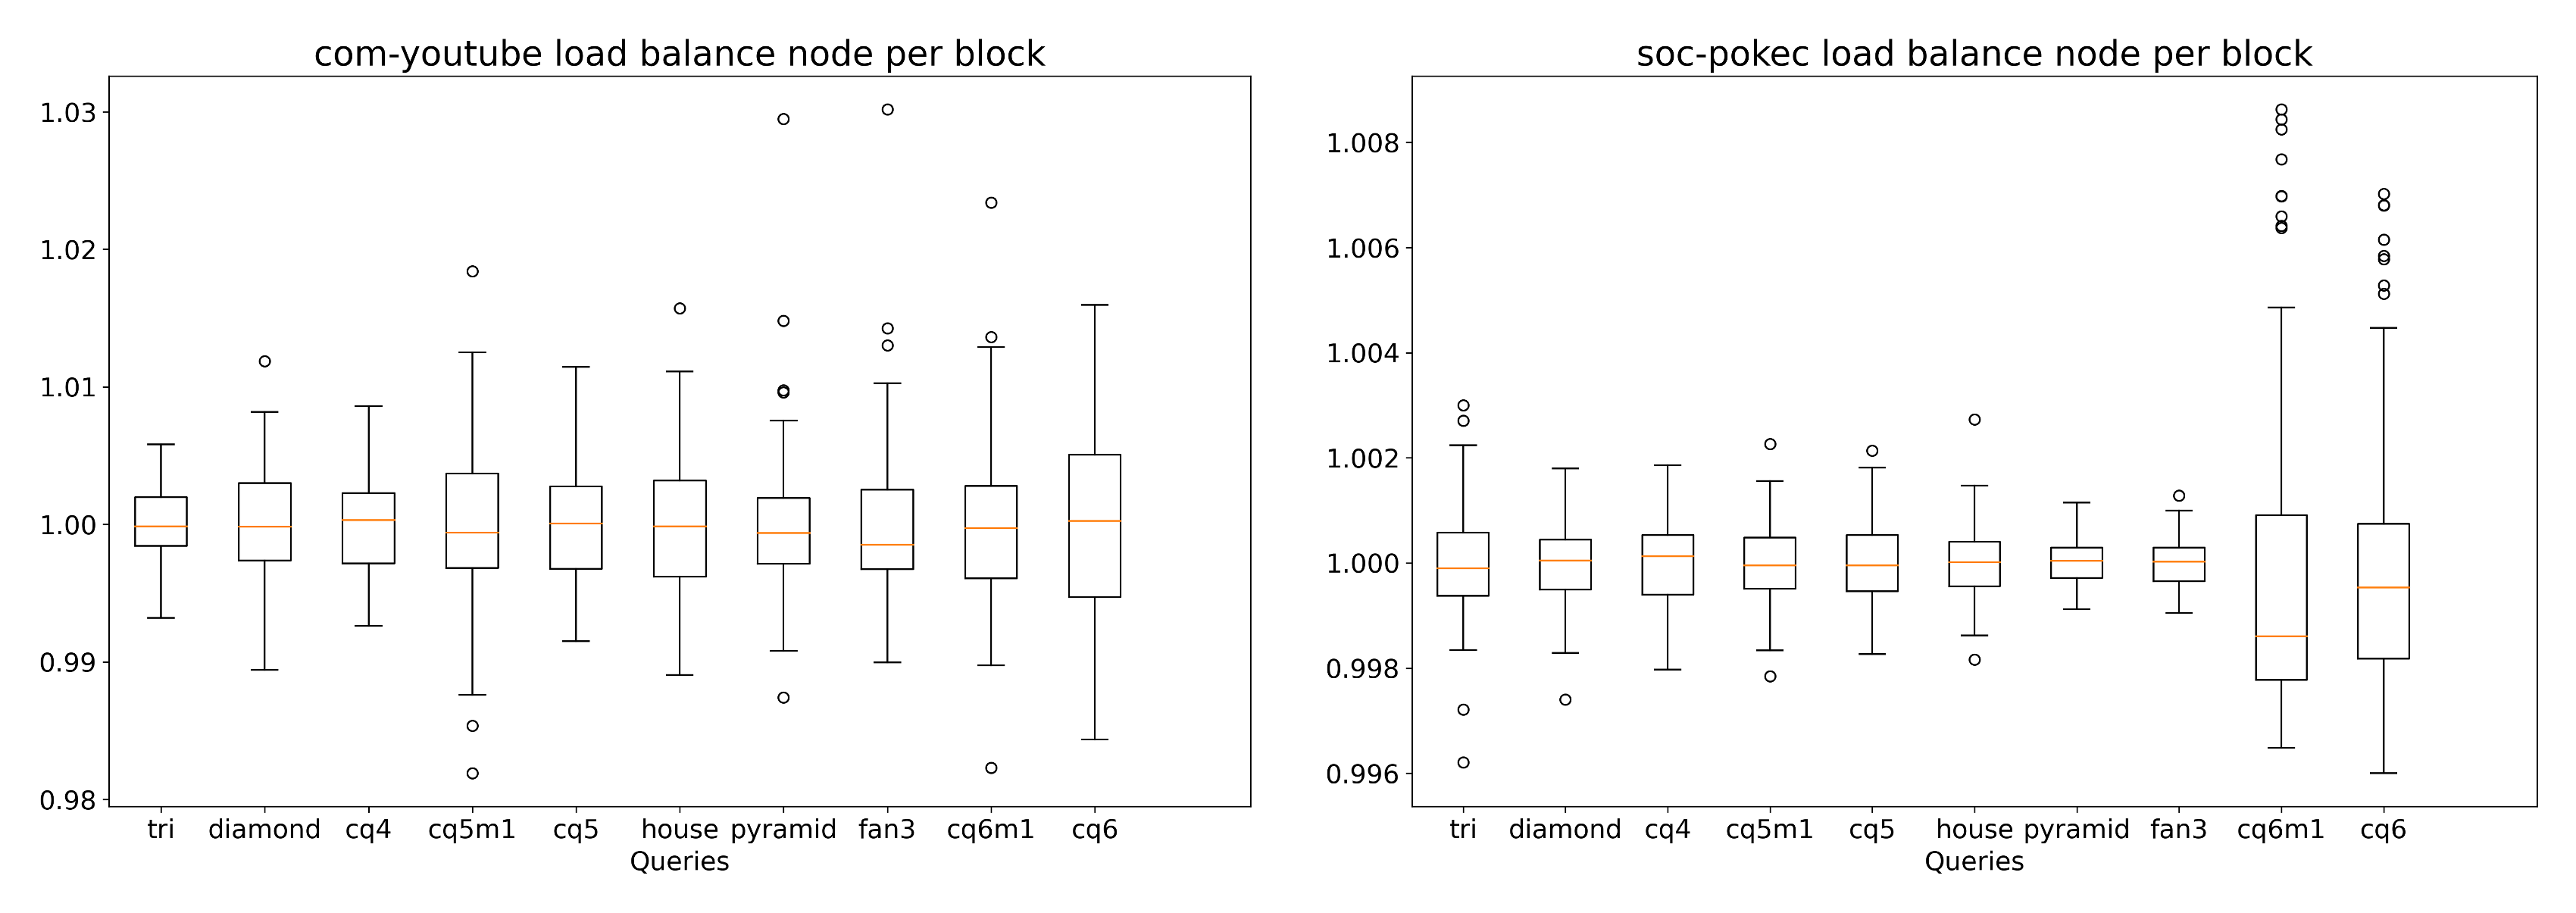
\includegraphics[width=\textwidth]{fig/improvements/load-balance-LD.png}
%     \caption{Load balance for nodes with degree $\leq 256$ }
%     \label{fig:load-balance-LD}
% \end{figure}

The claim from the authors of \cite{PARSEC_VD} was edge per block scheme works better than node per block for queries of size greater than five.
One reason for this claim is implied by the load balance observations above. However, it does not explain the slow performance of the edge per block kernel.
The reason is strictly based on the implementation. For the edge per block scheme in \cite{PARSEC_VD}, each block induces its own subgraph.
This causes extra workload hence the edge per block implementation outperforms only for larger query graphs as they exhibit worse load balance.

To eliminate this redundant work, the kernel is split into two parts with different parallelization schemes.
The first kernel ensures non-redundancy while inducing subgraphs by using the node per block scheme.
The second kernel uses these induced subgraphs to perform search tree traversal using the edge per block scheme while ensuring better load balance.
Since the kernels are split, the persistent memory technique needs to be removed.
To minimize the total number of kernel launches and better resource utilization a runtime query is made to the device memory to find the number of nodes that can be simultaneously processed.

It is clear from Figure \ref{fig:load-balance-LD} that low degree node processing is fairly load balanced with the node per block parallelization scheme.
Since splitting the kernels causes poor caching performance and launch overheads, a cutoff scheme was developed.
Nodes with degree less than cutoff would perform subgraph induction and search tree traversal in node per block fashion.
Whereas nodes with degree higher than cutoff would perform these operations in separate kernels as mentioned above.
Empirical testing was conducted to fix a cutoff value across different queries.
It was found that for dense queries like \textit{cqx} and \textit{cqxm1} cutoff value between $(1024 - 2048)$ is better while for sparse queries like \textit{fans} and \textit{wheels} cutoff value around $768$ achieved best results.
It was also observed that the run time is not too sensitive to cutoff.
Figure \ref{fig:cutoff-tests} shows the relative run times across different cutoffs.
Using these insights the cutoff was decided at runtime based on the input query.

\begin{figure}[h]
    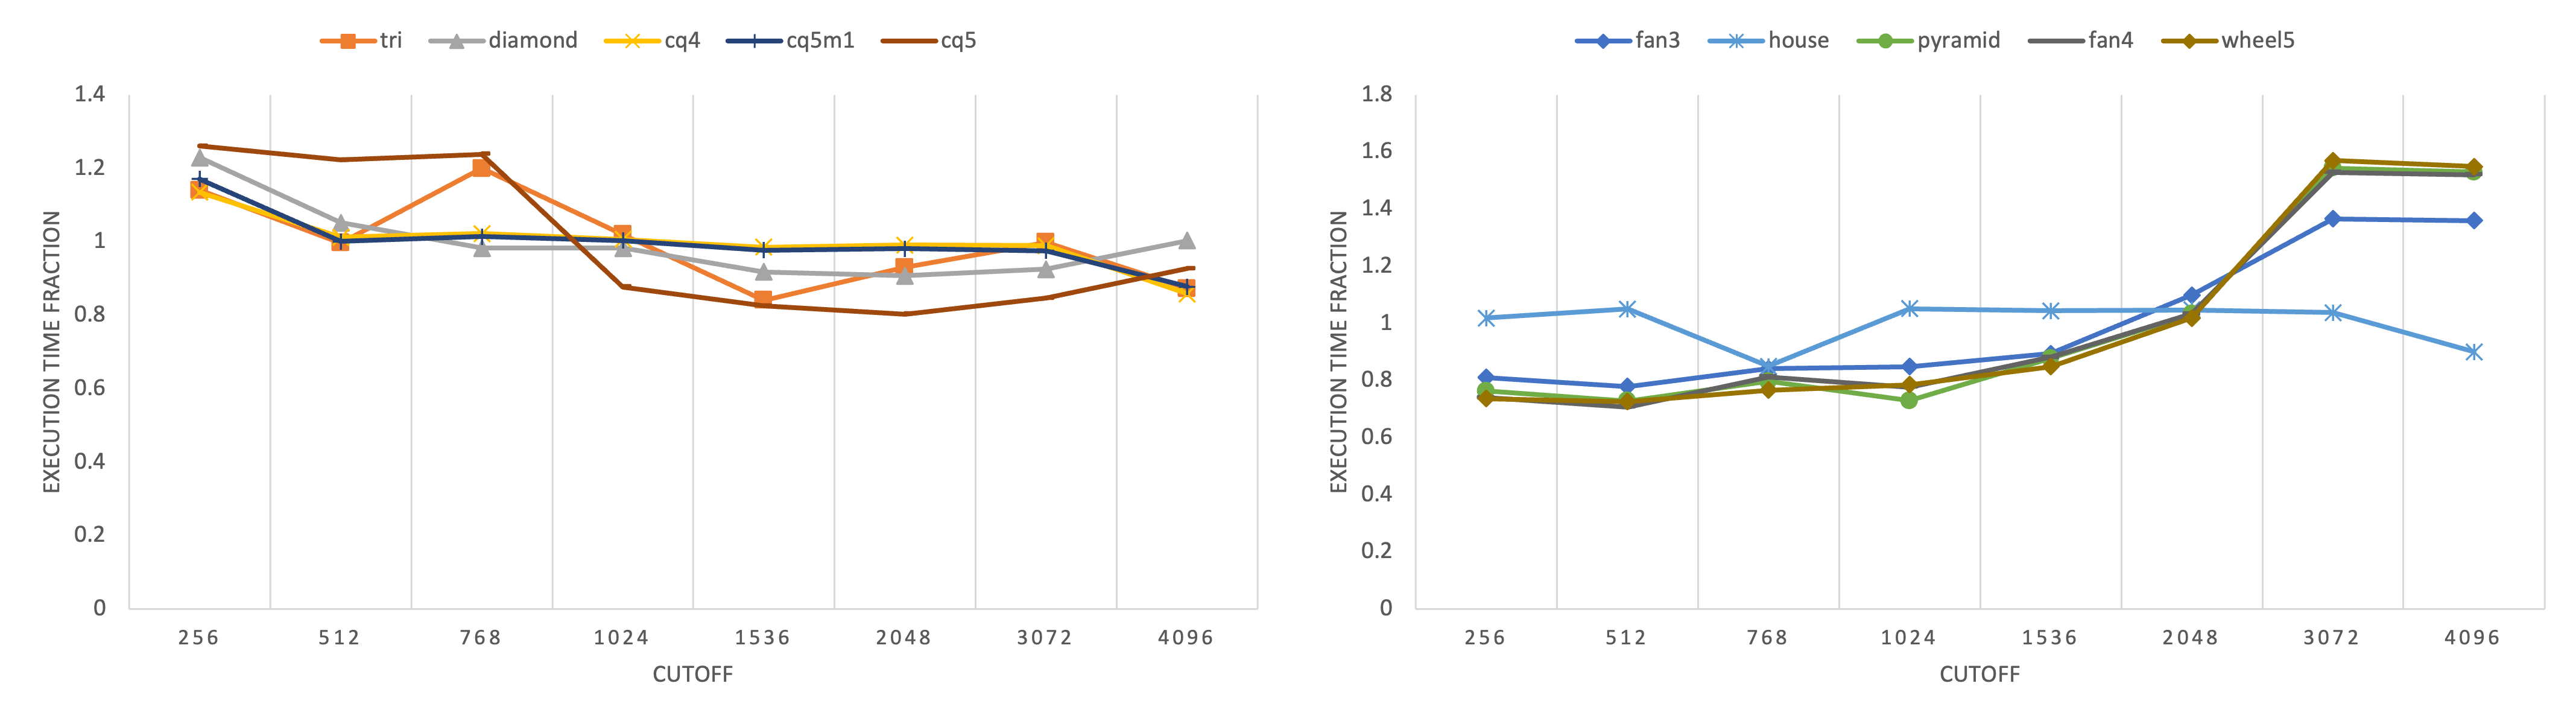
\includegraphics[width=\textwidth]{fig/improvements/cutoff-tests-yt.png}
    \caption{Run time fractions vs cutoff for com-youtube}
    \label{fig:cutoff-tests}
\end{figure}

Figure \ref{fig:hybrid-par-speedups} shows the improvement in runtimes for the com-youtube data graph across different queries.

\begin{figure}[h]
    \centering
    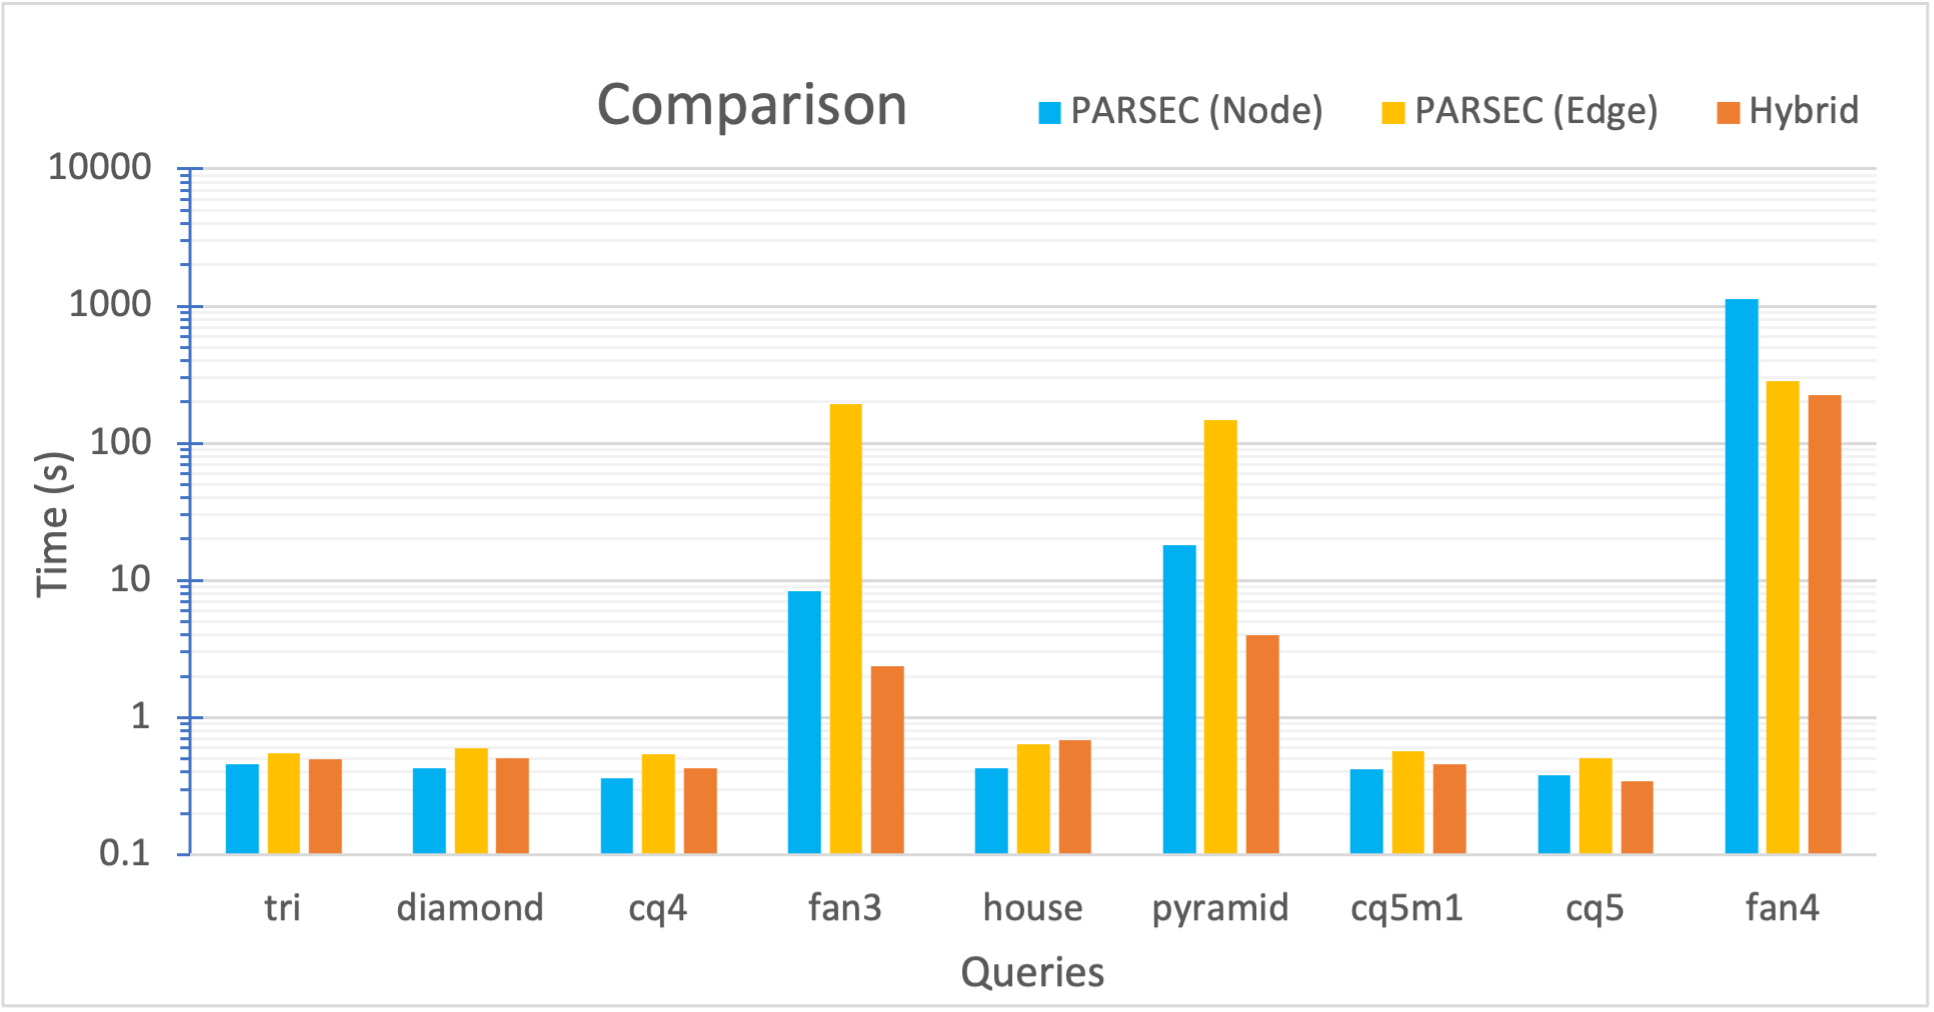
\includegraphics[width=0.6\textwidth]{fig/improvements/Hybrid-parallelism-speedups.png}
    \caption{Run times with Hybrid parallelism for com-youtube}
    \label{fig:hybrid-par-speedups}
\end{figure}
